\documentclass[landscape,a0paper,fontscale=0.285]{baposter} % Adjust the font scale/size here

\usepackage{graphicx} 
\graphicspath{{figures/}} % Directory in which figures are stored
\usepackage{amsmath} 
\usepackage{amssymb} 
\usepackage{booktabs} % Top and bottom rules for tables
\usepackage{enumitem} 
\usepackage{palatino} % Use the Palatino font
\usepackage[font=small,labelfont=bf]{caption} 
\usepackage{multicol} 
\setlength{\columnsep}{1.5em}
\setlength{\columnseprule}{0mm} 
\usepackage{tikz} 
\usetikzlibrary{shapes,arrows} 

\newcommand{\compresslist}{ 
  \setlength{\itemsep}{1pt}
  \setlength{\parskip}{0pt}
  \setlength{\parsep}{0pt}}
\newcommand{\bfSigma}{\mbox{\boldmath$\Sigma$}}
\newcommand{\bfLambda}{\mbox{\boldmath$\Lambda$}}
\DeclareMathOperator*{\argmax}{\arg\!\max}

\definecolor{lightblue}{rgb}{0.145,0.6666,1} 

\begin{document}

\begin{poster}
{
headerborder=closed, % Adds a border around the header of content boxes
colspacing=1em, % Column spacing
bgColorOne=white, % Background color for the gradient on the left side of the poster
bgColorTwo=white, % Background color for the gradient on the right side of the poster
borderColor=lightblue, % Border color
headerColorOne=black, % Background color for the header in the content boxes (left side)
headerColorTwo=lightblue, % Background color for the header in the content boxes (right side)
headerFontColor=white, % Text color for the header text in the content boxes
boxColorOne=white, % Background color of the content boxes
textborder=roundedleft, % Format of the border around content boxes, can be: none, bars, coils, triangles, rectangle, rounded, roundedsmall, roundedright or faded
eyecatcher=true, % Set to false for ignoring the left logo in the title and move the title left
headerheight=0.1\textheight, % Height of the header
headershape=roundedright, % Specify the rounded corner in the content box headers, can be: rectangle, small-rounded, roundedright, roundedleft or rounded
headerfont=\Large\bf\textsc, % Large, bold and sans serif font in the headers of content boxes
%textfont={\setlength{\parindent}{1.5em}}, % Uncomment for paragraph indentation
linewidth=2pt % Width of the border lines around content boxes
}
%----------------------------------------------------------------------------------------
%	TITLE SECTION 
%----------------------------------------------------------------------------------------
{
\includegraphics[height=3em]{milalogo}} 
{\bf\textsc{Applying LSTM to text generation}\vspace{0.5em}} % Poster title
{\textsc{J. Leroux, N. Laliberte, S. Frederic Boileau \hspace{5pt}\hspace{5pt} }}
{
\includegraphics[height=3em]{udemlogo}} % Second university/lab logo on the right

%----------------------------------------------------------------------------------------
%	STABILITY SELECTION
%----------------------------------------------------------------------------------------
\headerbox{Recurrent Neural Networks}{name = rnn, column = 0, span = 2}{

\begin{multicols}{2}
Recurrent neural networks (RNN) are a family of neural networks specialized for
processing a sequence of values. They are feedforward neural networks with the
addition of time dependency in the model by introducing edges that span the
adjacent time steps in the network. At a given time, the nodes with recurrent
edges receive input from the current data and from the output of the hidden
layer in the previous state, see figure below. Thus, an input at time $t$ can
influence the output at time $t + \delta$ by way of recurrent connections.

\begin{center}
    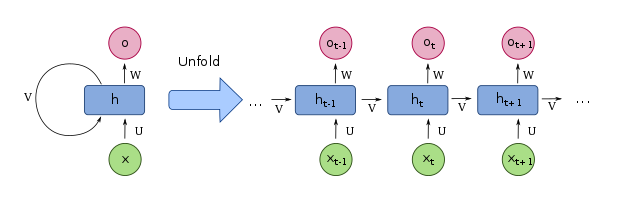
\includegraphics[width = 0.9\linewidth]{RNN.png}
\end{center}

Each time step are computed as follows:
\begin{align*}
    &h_t = \sigma(U x_t + V h_{(t-1)} + b_h)\text{,}\\
    &o_t = \text{softmax}(W h_t + b_o)
\end{align*}

Here, $ U$, $V$ and $W$ are weights matrix. The vectors $b$ are bias
parameters. Learning with RNN is challenging due to dependencies between long
time steps. Consider the gradient with respect to $h_t$ of $o_{t + \delta}$.
How does it vary with $\delta$? Following the graph above and applying the
chain rule we can see that
\begin{align*}
    \nabla_{h_t}o_{t + \delta} =
    \left( \prod_{k = t+1}^{t+\delta} V^T \text{diag}(1 - h^2_k) \right)
    \nabla_{h_{t + \delta}}o_{t + \delta}.
\end{align*}

Thus, as $\delta$ grows, the gradient grows exponentially with $V$. If $V$ is
small or large than the gradient will either vanish or explode. This problem is
well known. Solutions exist, which brings us to present the Long Short-Term
Memory network (LSTM).

\end{multicols}
}%headerbox

%%%%%%%%%%%%%%%%%%%%%%%%%%%%%%%%%%%%%%%%%%%%%%%%%%%%%%%%%%%%%%%%%%%%%%%%%%%%%%%
\headerbox{LSTM}{name = lstm, column = 0, below = rnn, above = bottom, span = 2}{

\begin{multicols}{2}
The LSTM model has been introduced primarily to solve the vanishing and
exploding gradients problem. This model is a RNN in which we replaced every
hidden nodes by a \textit{memory cell}.

\begin{center}
    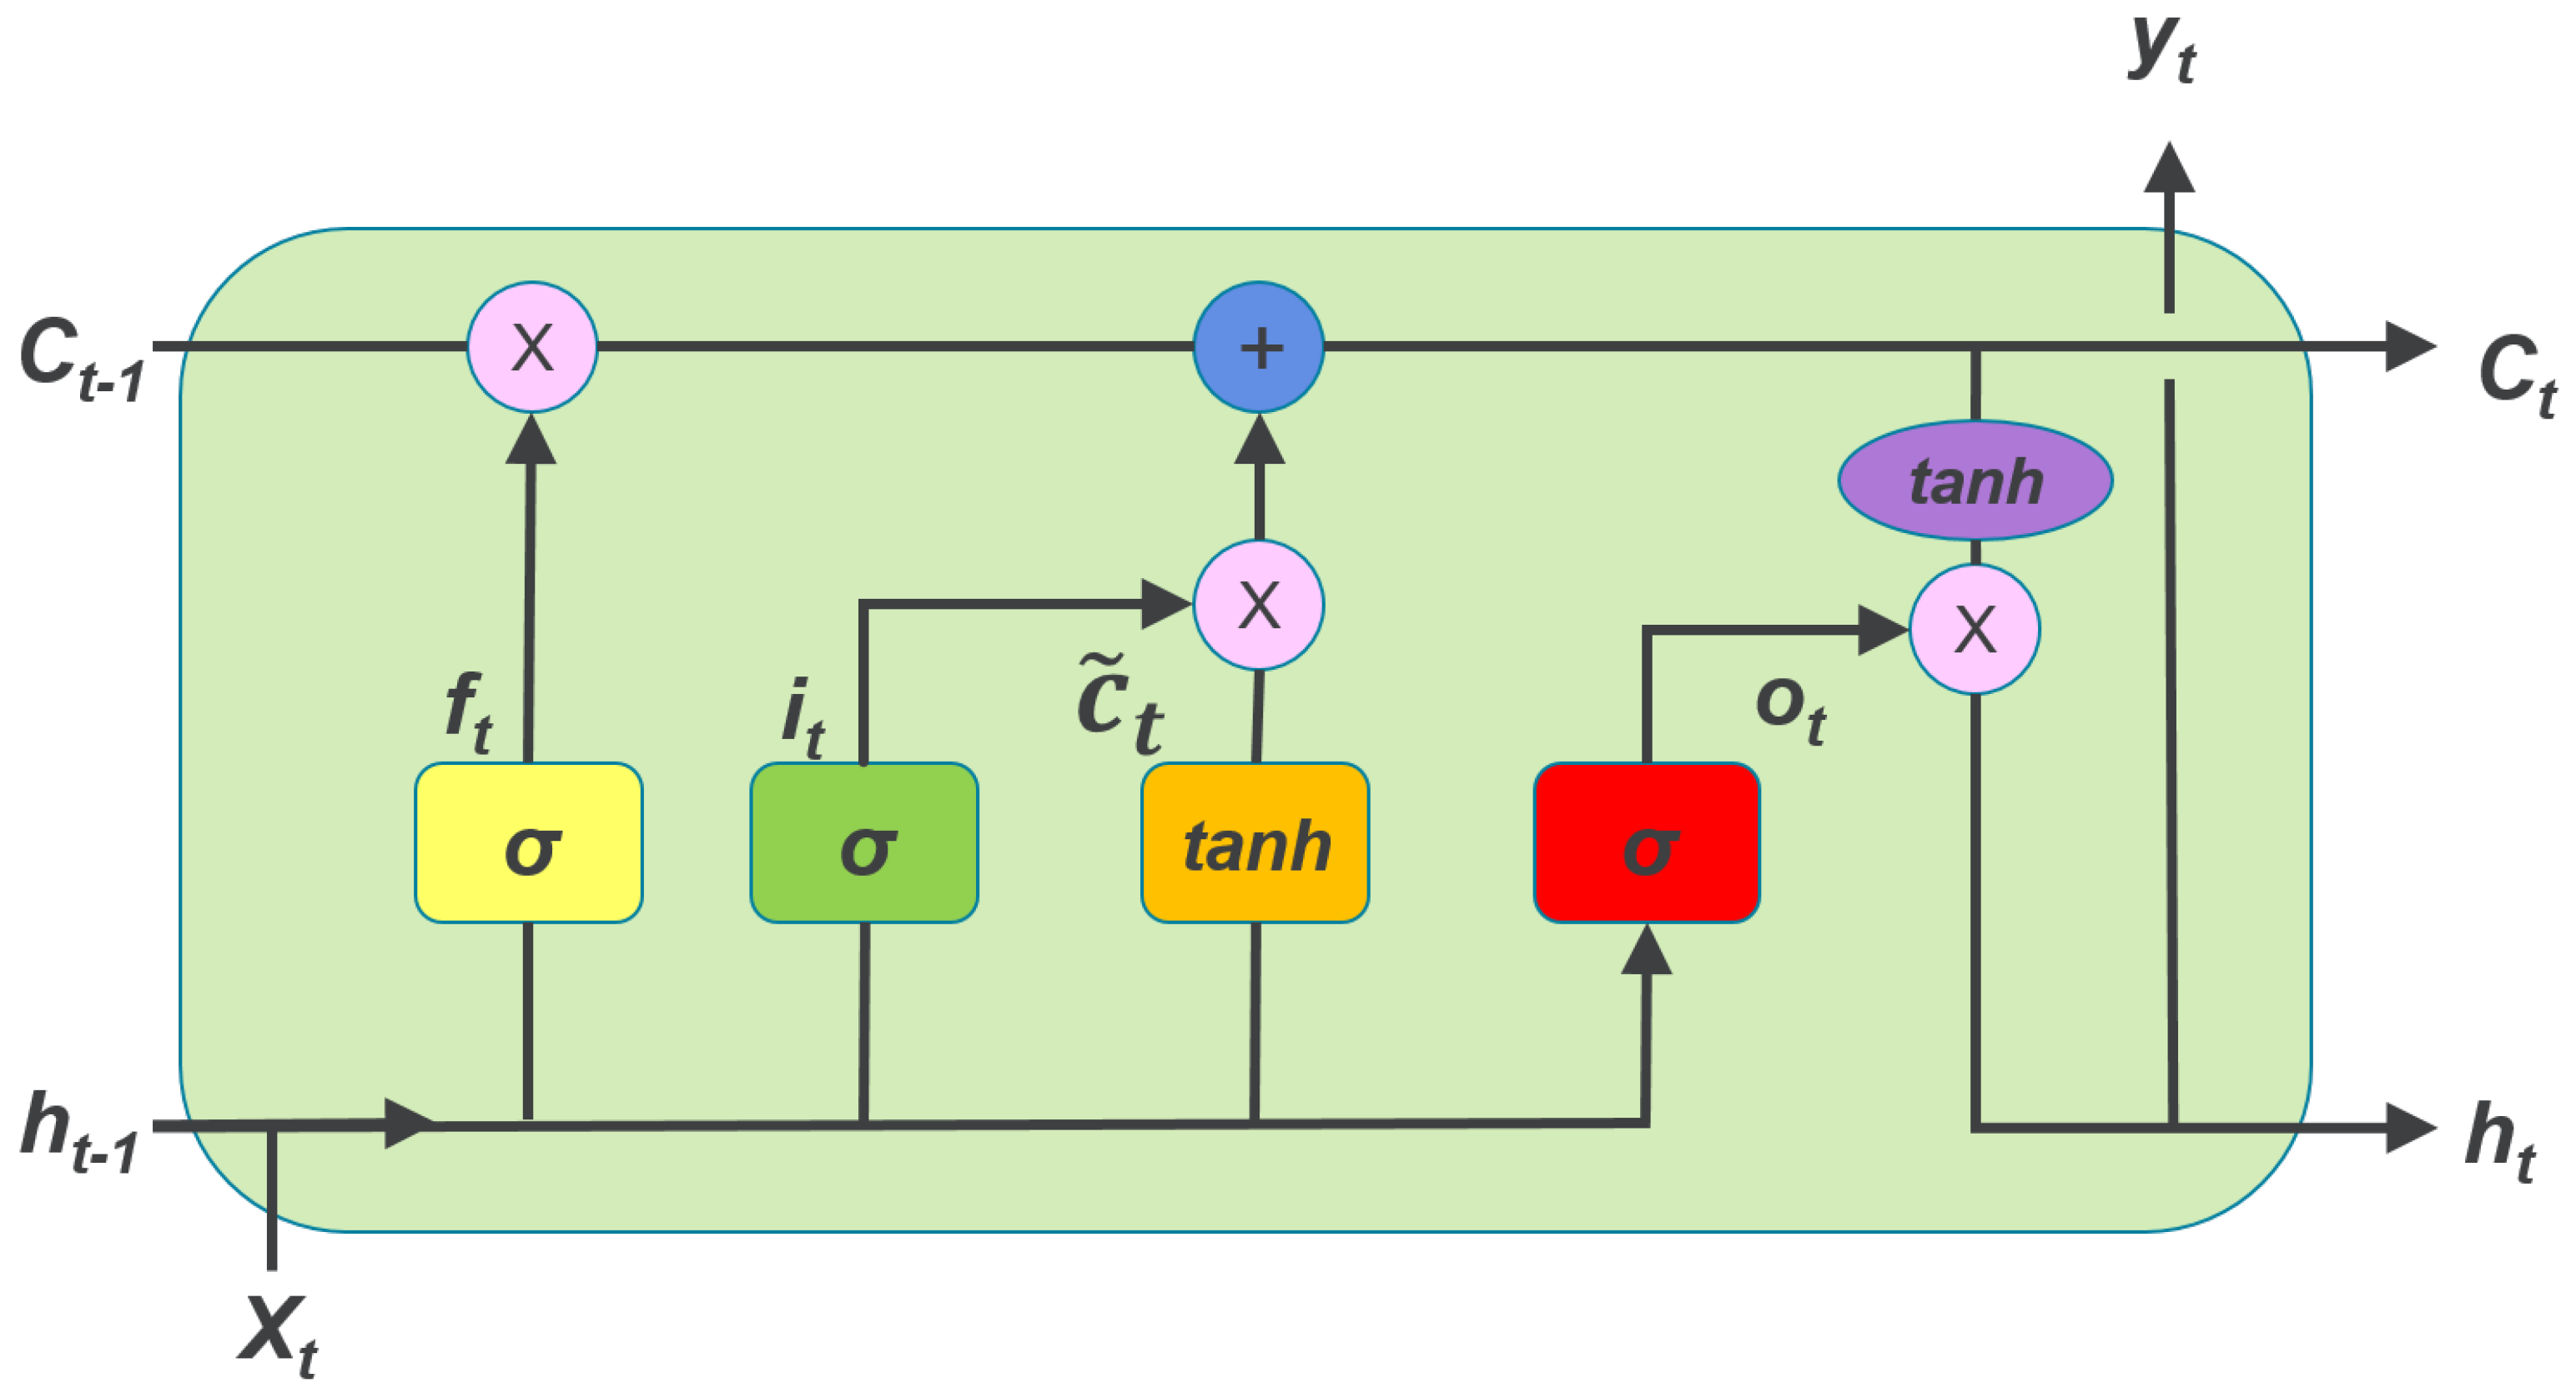
\includegraphics[width = 0.7\linewidth]{lstm.png}
\end{center}

Intuitively, RNN have \textit{long-term memory} in the form of matrix weights,
they change during the training encoding general knowledge about the data. RNN
also have \textit{short-term memory} in the form of activation passing from
each node to successive ones. The memory cell introduced in the LSTM model
provides storage for those memories. We now describe components of the cell.

\begin{center}
    \begin{itemize}
    \item Gates ($f_t, i_t, c_t$): They are sigmoidal units that takes
      activation from the input $x_t$ and the output of the hidden layer from
      previous state $h_{t-1}$. Note that $f_t$ multiply the value of the
      previous cell $c_{t-1}$. The term \textit{gate} stands for the literal
      meaning in the sense that if $f_{t}$ is close to $0$, then the gate is
      \textit{closed} and the flow from the previous cell is cut off. If $f_t$
      is closed to $1$ then all flow is passed through.
    
    \item Cell state ($c_t = f_t \cdot c_{t-1} + i_t \cdot \tilde{c}_t$): Cell
  state maintains information on the input. Also refered as the internal state,
  $c_t$ has a self-connected edges with a fixed unit weight. This constant
  weight implies that the error can flow across time without vanishing or
  exploding.  \end{itemize}
\end{center}
\end{multicols}
}%headerbox


%----------------------------------------------------------------------------------------
%	SIMULATION STUDY 
%----------------------------------------------------------------------------------------
\headerbox{Results}{name = results, column = 2 ,span = 2, row = 0}{
\vspace{0.05 cm}
\subsection*{Implemented network}

\begin{multicols}{2}
For the implementation section of this projet, we decided to use Recurent
Neural Network, more specificaly LSTM, for the generation and the
classification of sequential data. More concretely, we gathered text data that
we found around the internet to train a sequence classifier. The training of
the classifier consist of identifying from which corpus between Harry Potter,
Lord of the rings, some random quotes and Shakespeare, the sequence corresponds
to. Further to this, we trained one model per sequence type for the text
generation. Finally, we verified that our generated sequences were well
classified by our classifier.

\begin{center}
\begin{tabular}{|l|l|l|}
\hline
Parameters & Classification & TextGen \\
\hline
Input dim & 60k & 60k \\
Embedding dim & 256 & 256 \\
Hidden/cell dim & 256 & 512 \\
Output dim & 4 & 60k\\
\hline
\end{tabular}
\end{center}

\subsection*{Preprocessing and model details}
Before doing any sort or training, we had to do a bit of preprocessing on the
data. First, we tokenized each corpus in sequences of 50 tokens.
\end{multicols}
\begin{multicols}{2}
%\begin{center}
%\subsection*{Classification of sequences}
%\begin{center}
	%\includegraphics[width=.65\linewidth]{}
%\end{center}
%\end{center}
%\begin{center}
%\includegraphics[width=.65\linewidth]{}
%\end{center}
%------------------------------------------------
\begin{center}
\subsection*{TextGen and Classification}
\end{center}
%\begin{center}
	%\includegraphics[width=.95\linewidth]{}
%\end{center}
The architecture we used for the text generation is of the form of a many-to-many LSTM. For the training, the corpus was separated in sequences of 50 tokens
\begin{itemize}\compresslist
    \item `` well , we ' ll do it with a wand , '' said hermione . `` really ? '' said harry , looking at each other .
    \item  what looked about this way , the black citadel , was far from the darkness , the ring was heard , but the sea big was big , and a great ring was in his battle .
    \item failure is a beginning of love and a family which comes from god .
    \item  '' that now my mind shall screens his music , '' '' and i to give thee my vulgar heaven , '' '' i am your brother .
\end{itemize}
\end{multicols} }

\vspace{-1 cm}

%\begin{center}
%\subsection*{Conclusion}
%\end{center}

% When there are two boxes, some whitespace may need to be added if the one on the right has more content

%----------------------------------------------------------------------------------------
%	REFERENCES
%----------------------------------------------------------------------------------------
\headerbox{References}{name=ref, column = 2, span = 2, below = results, above = bottom}{

\begin{enumerate}
    \item Zachary Chase Lipton, 2015. A Critical Review of Recurrent Neural Networks for Sequence Learning, CoRR. 
\end{enumerate}

}%headebox
%----------------------------------------------------------------------------------------
%	CONCLUSION 
%----------------------------------------------------------------------------------------
%\headerbox{Further Work}{name=conclusion,column=2,span=2,below=CLSA,above=bottom}{

%\begin{itemize}\compresslist
%\item Exploration and development of loss functions on unknown graph structure is a relevant idea.
%\end{itemize}
%\vspace{0.3em} % When there are two boxes, some whitespace may need to be added if the one on the right has more content
%}
\end{poster}
\end{document}
